\section*{Problem 2.1: A Simple Power Supply}
A simple power supply is presented for analysis. 
\begin{figure}[H]
    \centering
    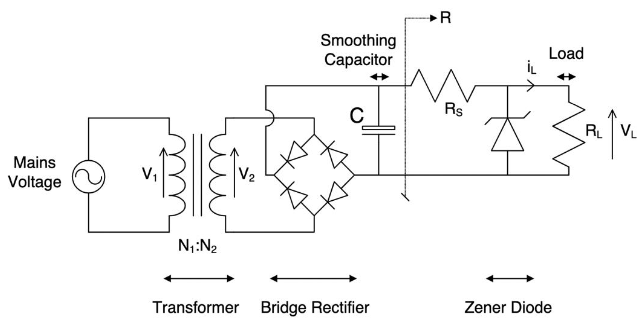
\includegraphics[width=\textwidth]{graphics/powersupply.png}
    \caption{Simple power supply}
    \label{fig:powersupply}
\end{figure}
The power supply is terminated by a multi-mode load resistor modelled by its Thevenin equivalent circuit. The circuit has multiple modes of operation depending on the switching of its devices. The circuit is presented below.
\begin{figure}[H]
    \centering
    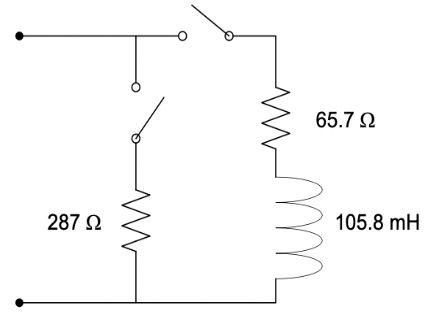
\includegraphics[width=8cm]{graphics/multimode_load.png}
    \caption{Multi-mode load}
    \label{fig:multimode_load}
\end{figure}
The performance of the circuit is to be determined for all modes of operation. A mathematical model of the circuit is derived for use in numerical analysis and simulation. A visualisation is presented at the end with the results.